\subsection{Question 1}
Le système d'impression de pièces peut etre modéliser par le réseaux suivant :
\begin{figure}[H]
  \centering
  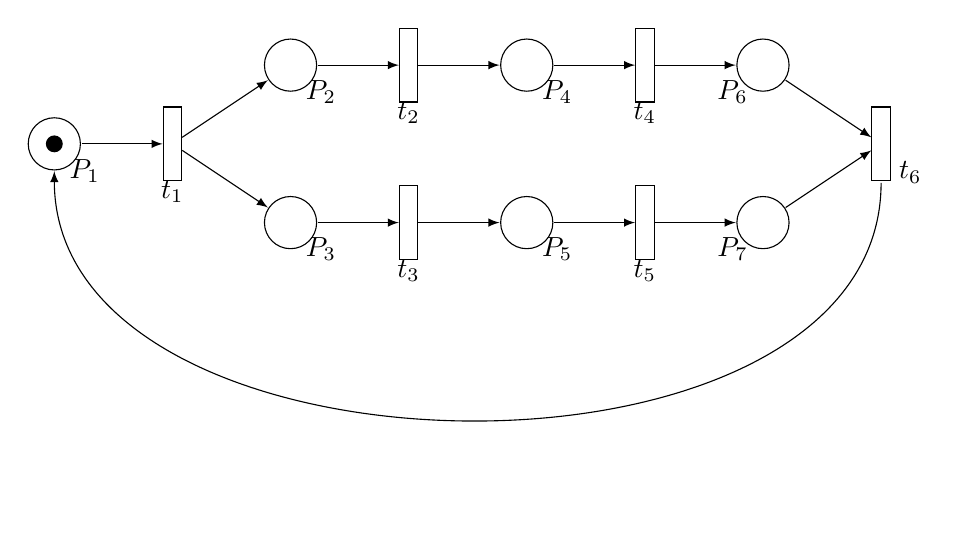
\begin{tikzpicture}
    % Liste des places
    \draw (-6,0) node[below right = 2pt] {$P_1$};
    \node[draw,circle,scale=2] (P1) at (-6, 0) {};
    \draw (-3,1) node[below right = 2pt] {$P_2$};
    \node[draw,circle,scale=2] (P2) at (-3, 1) {};
    \draw (-3,-1) node[below right = 2pt] {$P_3$};
    \node[draw,circle,scale=2] (P3) at (-3,-1) {};
    \draw (0,1) node[below right = 2pt] {$P_4$};
    \node[draw,circle,scale=2] (P4) at (0, 1) {};
    \draw (0,-1) node[below right = 2pt] {$P_5$};
    \node[draw,circle,scale=2] (P5) at (0,-1) {};
    \draw (3,1) node[below left = 2pt] {$P_6$};
    \node[draw,circle,scale=2] (P6) at (3, 1) {};
    \draw (3,-1) node[below left = 2pt] {$P_7$};
    \node[draw,circle,scale=2] (P7) at (3,-1) {};

    % Liste des transitions
    \draw (-4.5,0) node[below = 10pt] {$t_1$};
    \node[draw,rectangle,yscale=4] (t1) at (-4.5, 0) {};
    \draw (-1.5,-1) node[below = 10pt] {$t_3$};
    \node[draw,rectangle,yscale=4] (t3) at (-1.5, -1) {};
    \draw (-1.5,1) node[below = 10pt] {$t_2$};
    \node[draw,rectangle,yscale=4] (t2) at (-1.5, 1) {};
    \draw (1.5,-1) node[below = 10pt] {$t_5$};
    \node[draw,rectangle,yscale=4] (t5) at (1.5, -1) {};
    \draw (1.5,1) node[below = 10pt] {$t_4$};
    \node[draw,rectangle,yscale=4] (t4) at (1.5, 1) {};
    \draw (4.5,0) node[below right = 3pt] {$t_6$};
    \node[draw,rectangle,yscale=4] (t6) at (4.5, 0) {};

    % Liste des arcs
    \draw[->,>=latex] (P1) -- (t1);
    \draw[->,>=latex] (t1) -- (P2);
    \draw[->,>=latex] (t1) -- (P3);
    \draw[->,>=latex] (P3) -- (t3);
    \draw[->,>=latex] (P2) -- (t2);
    \draw[->,>=latex] (t2) -- (P4);
    \draw[->,>=latex] (t3) -- (P5);
    \draw[->,>=latex] (P4) -- (t4);
    \draw[->,>=latex] (P5) -- (t5);
    \draw[->,>=latex] (t4) -- (P6);
    \draw[->,>=latex] (t5) -- (P7);
    \draw[->,>=latex] (P6) -- (t6);
    \draw[->,>=latex] (P7) -- (t6);
    \draw[->,>=latex] (t6) to[out=-90,in=-90] (P1);

    % Marquage 
    \draw [fill](-6,0) circle (0.1) ;
  \end{tikzpicture}
  \caption{Réseau de petri associé au système d'impréssion par pochoir} \label{fig:M1}
\end{figure}

\subsection{Question 2}
Faisons tourner le système, à l'état initiale nous avons le réseau de la figure 1.\\
Lorsque la pièce est insérer dans le système et que les pochoirs sont prêt, le signal $p \wedge q$ est envoyé :

\begin{figure}[H]
  \centering
  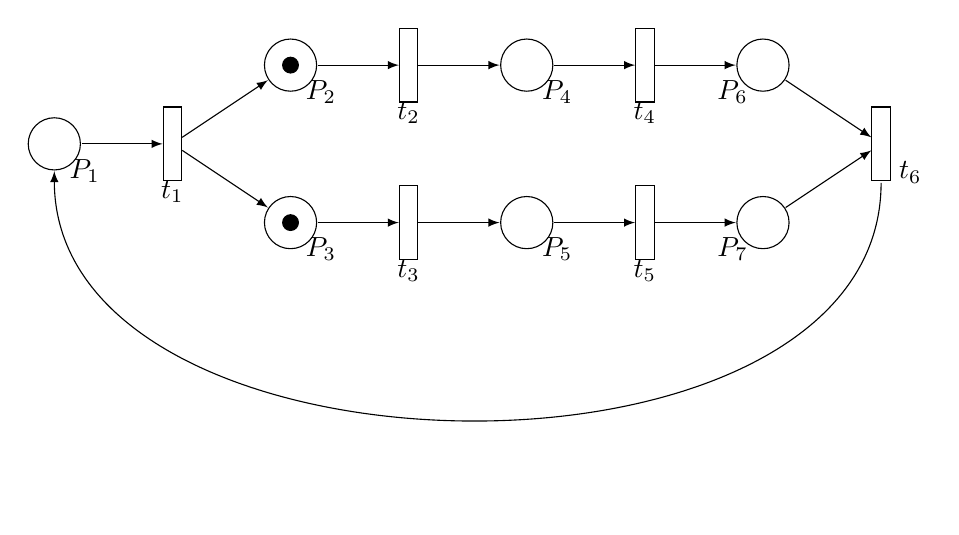
\begin{tikzpicture}
    % Liste des places
    \draw (-6,0) node[below right = 2pt] {$P_1$};
    \node[draw,circle,scale=2] (P1) at (-6, 0) {};
    \draw (-3,1) node[below right = 2pt] {$P_2$};
    \node[draw,circle,scale=2] (P2) at (-3, 1) {};
    \draw (-3,-1) node[below right = 2pt] {$P_3$};
    \node[draw,circle,scale=2] (P3) at (-3,-1) {};
    \draw (0,1) node[below right = 2pt] {$P_4$};
    \node[draw,circle,scale=2] (P4) at (0, 1) {};
    \draw (0,-1) node[below right = 2pt] {$P_5$};
    \node[draw,circle,scale=2] (P5) at (0,-1) {};
    \draw (3,1) node[below left = 2pt] {$P_6$};
    \node[draw,circle,scale=2] (P6) at (3, 1) {};
    \draw (3,-1) node[below left = 2pt] {$P_7$};
    \node[draw,circle,scale=2] (P7) at (3,-1) {};

    % Liste des transitions
    \draw (-4.5,0) node[below = 10pt] {$t_1$};
    \node[draw,rectangle,yscale=4] (t1) at (-4.5, 0) {};
    \draw (-1.5,-1) node[below = 10pt] {$t_3$};
    \node[draw,rectangle,yscale=4] (t3) at (-1.5, -1) {};
    \draw (-1.5,1) node[below = 10pt] {$t_2$};
    \node[draw,rectangle,yscale=4] (t2) at (-1.5, 1) {};
    \draw (1.5,-1) node[below = 10pt] {$t_5$};
    \node[draw,rectangle,yscale=4] (t5) at (1.5, -1) {};
    \draw (1.5,1) node[below = 10pt] {$t_4$};
    \node[draw,rectangle,yscale=4] (t4) at (1.5, 1) {};
    \draw (4.5,0) node[below right= 3pt] {$t_6$};
    \node[draw,rectangle,yscale=4] (t6) at (4.5, 0) {};

    % Liste des arcs
    \draw[->,>=latex] (P1) -- (t1);
    \draw[->,>=latex] (t1) -- (P2);
    \draw[->,>=latex] (t1) -- (P3);
    \draw[->,>=latex] (P3) -- (t3);
    \draw[->,>=latex] (P2) -- (t2);
    \draw[->,>=latex] (t2) -- (P4);
    \draw[->,>=latex] (t3) -- (P5);
    \draw[->,>=latex] (P4) -- (t4);
    \draw[->,>=latex] (P5) -- (t5);
    \draw[->,>=latex] (t4) -- (P6);
    \draw[->,>=latex] (t5) -- (P7);
    \draw[->,>=latex] (P6) -- (t6);
    \draw[->,>=latex] (P7) -- (t6);
    \draw[->,>=latex] (t6) to[out=-90,in=-90] (P1);

    % Marquage 
    \draw [fill](-3,1) circle (0.1) ;
    \draw [fill](-3,-1) circle (0.1) ;
  \end{tikzpicture}
  \caption{Réseau après initialisation du système} \label{fig:M2}
\end{figure}

\newpage

On peut ensuite faire avancer le pochoir droit (fig. 3) ou gauche (fig.4) :

\begin{figure}[H]
  \centering
  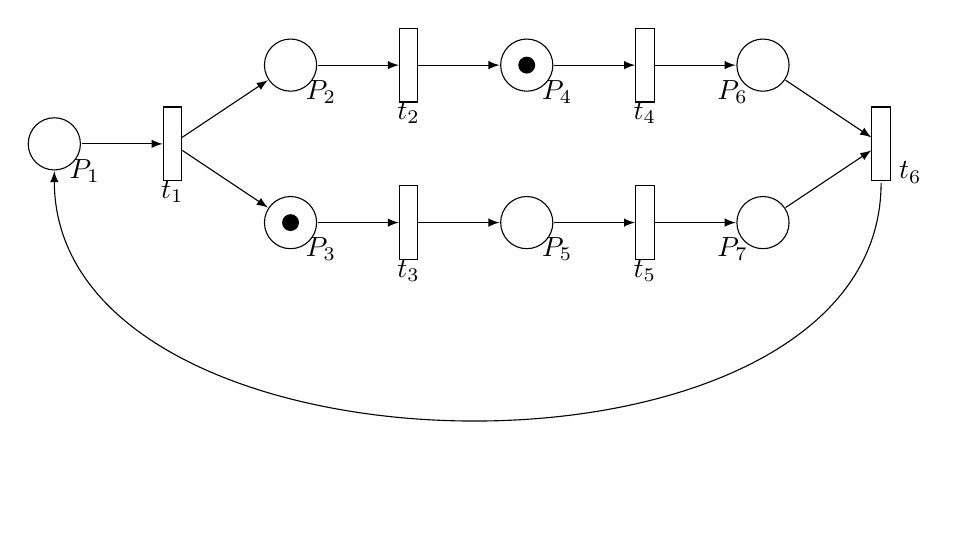
\begin{tikzpicture}
    % Liste des places
    \draw (-6,0) node[below right = 2pt] {$P_1$};
    \node[draw,circle,scale=2] (P1) at (-6, 0) {};
    \draw (-3,1) node[below right = 2pt] {$P_2$};
    \node[draw,circle,scale=2] (P2) at (-3, 1) {};
    \draw (-3,-1) node[below right = 2pt] {$P_3$};
    \node[draw,circle,scale=2] (P3) at (-3,-1) {};
    \draw (0,1) node[below right = 2pt] {$P_4$};
    \node[draw,circle,scale=2] (P4) at (0, 1) {};
    \draw (0,-1) node[below right = 2pt] {$P_5$};
    \node[draw,circle,scale=2] (P5) at (0,-1) {};
    \draw (3,1) node[below left = 2pt] {$P_6$};
    \node[draw,circle,scale=2] (P6) at (3, 1) {};
    \draw (3,-1) node[below left = 2pt] {$P_7$};
    \node[draw,circle,scale=2] (P7) at (3,-1) {};

    % Liste des transitions
    \draw (-4.5,0) node[below = 10pt] {$t_1$};
    \node[draw,rectangle,yscale=4] (t1) at (-4.5, 0) {};
    \draw (-1.5,-1) node[below = 10pt] {$t_3$};
    \node[draw,rectangle,yscale=4] (t3) at (-1.5, -1) {};
    \draw (-1.5,1) node[below = 10pt] {$t_2$};
    \node[draw,rectangle,yscale=4] (t2) at (-1.5, 1) {};
    \draw (1.5,-1) node[below = 10pt] {$t_5$};
    \node[draw,rectangle,yscale=4] (t5) at (1.5, -1) {};
    \draw (1.5,1) node[below = 10pt] {$t_4$};
    \node[draw,rectangle,yscale=4] (t4) at (1.5, 1) {};
    \draw (4.5,0) node[below right= 3pt] {$t_6$};
    \node[draw,rectangle,yscale=4] (t6) at (4.5, 0) {};

    % Liste des arcs
    \draw[->,>=latex] (P1) -- (t1);
    \draw[->,>=latex] (t1) -- (P2);
    \draw[->,>=latex] (t1) -- (P3);
    \draw[->,>=latex] (P3) -- (t3);
    \draw[->,>=latex] (P2) -- (t2);
    \draw[->,>=latex] (t2) -- (P4);
    \draw[->,>=latex] (t3) -- (P5);
    \draw[->,>=latex] (P4) -- (t4);
    \draw[->,>=latex] (P5) -- (t5);
    \draw[->,>=latex] (t4) -- (P6);
    \draw[->,>=latex] (t5) -- (P7);
    \draw[->,>=latex] (P6) -- (t6);
    \draw[->,>=latex] (P7) -- (t6);
    \draw[->,>=latex] (t6) to[out=-90,in=-90] (P1);

    % Marquage 
    \draw [fill](0,1) circle (0.1) ;
    \draw [fill](-3,-1) circle (0.1) ;
  \end{tikzpicture}
  \caption{Réseau après l'avancement du pochoir droit} \label{fig:M3}
\end{figure}

\begin{figure}[H]
  \centering
  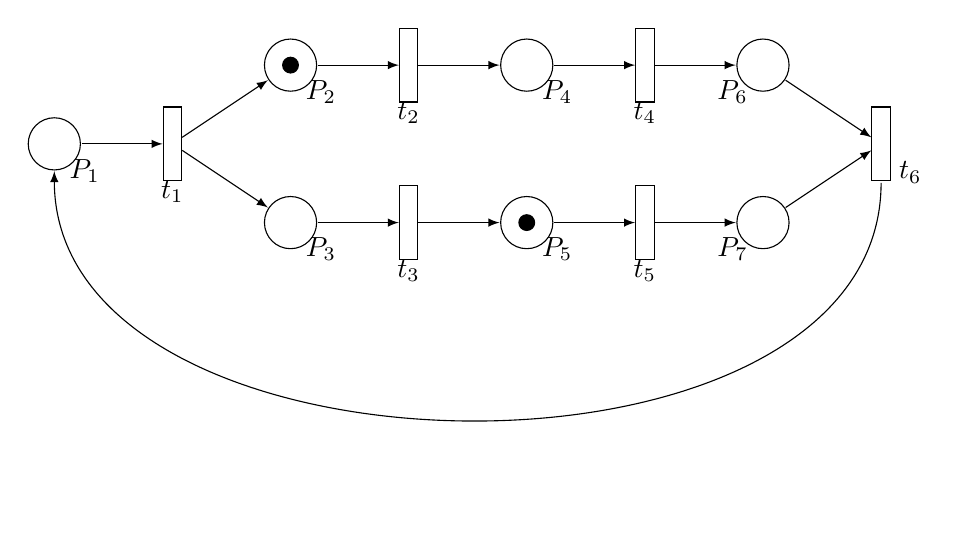
\begin{tikzpicture}
    % Liste des places
    \draw (-6,0) node[below right = 2pt] {$P_1$};
    \node[draw,circle,scale=2] (P1) at (-6, 0) {};
    \draw (-3,1) node[below right = 2pt] {$P_2$};
    \node[draw,circle,scale=2] (P2) at (-3, 1) {};
    \draw (-3,-1) node[below right = 2pt] {$P_3$};
    \node[draw,circle,scale=2] (P3) at (-3,-1) {};
    \draw (0,1) node[below right = 2pt] {$P_4$};
    \node[draw,circle,scale=2] (P4) at (0, 1) {};
    \draw (0,-1) node[below right = 2pt] {$P_5$};
    \node[draw,circle,scale=2] (P5) at (0,-1) {};
    \draw (3,1) node[below left = 2pt] {$P_6$};
    \node[draw,circle,scale=2] (P6) at (3, 1) {};
    \draw (3,-1) node[below left = 2pt] {$P_7$};
    \node[draw,circle,scale=2] (P7) at (3,-1) {};

    % Liste des transitions
    \draw (-4.5,0) node[below = 10pt] {$t_1$};
    \node[draw,rectangle,yscale=4] (t1) at (-4.5, 0) {};
    \draw (-1.5,-1) node[below = 10pt] {$t_3$};
    \node[draw,rectangle,yscale=4] (t3) at (-1.5, -1) {};
    \draw (-1.5,1) node[below = 10pt] {$t_2$};
    \node[draw,rectangle,yscale=4] (t2) at (-1.5, 1) {};
    \draw (1.5,-1) node[below = 10pt] {$t_5$};
    \node[draw,rectangle,yscale=4] (t5) at (1.5, -1) {};
    \draw (1.5,1) node[below = 10pt] {$t_4$};
    \node[draw,rectangle,yscale=4] (t4) at (1.5, 1) {};
    \draw (4.5,0) node[below right= 3pt] {$t_6$};
    \node[draw,rectangle,yscale=4] (t6) at (4.5, 0) {};

    % Liste des arcs
    \draw[->,>=latex] (P1) -- (t1);
    \draw[->,>=latex] (t1) -- (P2);
    \draw[->,>=latex] (t1) -- (P3);
    \draw[->,>=latex] (P3) -- (t3);
    \draw[->,>=latex] (P2) -- (t2);
    \draw[->,>=latex] (t2) -- (P4);
    \draw[->,>=latex] (t3) -- (P5);
    \draw[->,>=latex] (P4) -- (t4);
    \draw[->,>=latex] (P5) -- (t5);
    \draw[->,>=latex] (t4) -- (P6);
    \draw[->,>=latex] (t5) -- (P7);
    \draw[->,>=latex] (P6) -- (t6);
    \draw[->,>=latex] (P7) -- (t6);
    \draw[->,>=latex] (t6) to[out=-90,in=-90] (P1);

    % Marquage 
    \draw [fill](-3,1) circle (0.1) ;
    \draw [fill](0,-1) circle (0.1) ;
  \end{tikzpicture}
  \caption{Réseau après l'avancement du pochoir gauche} \label{fig:M4}
\end{figure}

A cet instant, on a plusieurs évolution du système possible : 
\begin{enumerate}
  \item Si le pochoir droit a été avancer : \\
    \begin{itemize}
      \item On peut alors le reculer : fig. 7
      \item On peut avancer le pochoir gauche : fig. 5
    \end{itemize}
  \item Si le pochoir gauche a été avancer : \\
    \begin{itemize}
      \item On peut alors le reculer : fig. 6
      \item On peut avancer le pochoir droit : fig. 5
    \end{itemize}
\end{enumerate}

\begin{figure}[H]
  \centering
  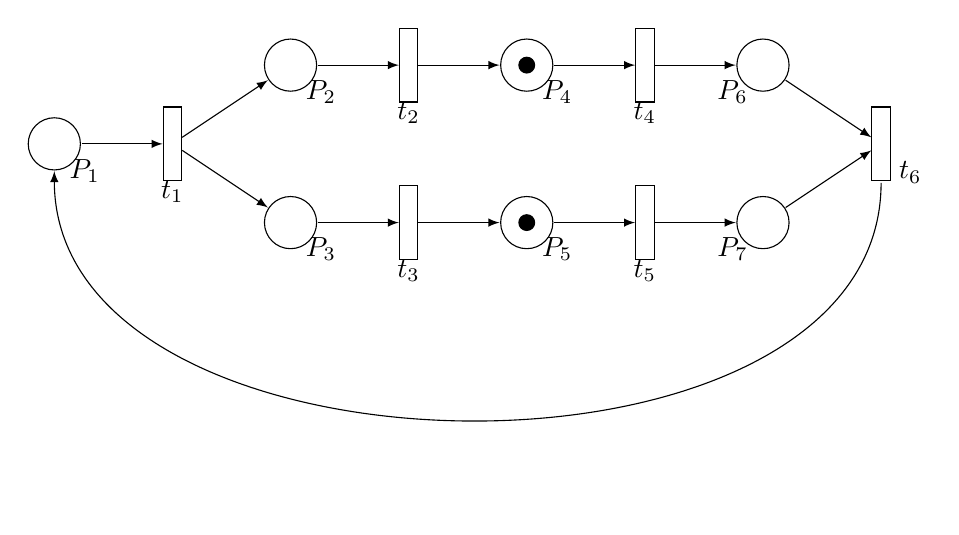
\begin{tikzpicture}
    % Liste des places
    \draw (-6,0) node[below right = 2pt] {$P_1$};
    \node[draw,circle,scale=2] (P1) at (-6, 0) {};
    \draw (-3,1) node[below right = 2pt] {$P_2$};
    \node[draw,circle,scale=2] (P2) at (-3, 1) {};
    \draw (-3,-1) node[below right = 2pt] {$P_3$};
    \node[draw,circle,scale=2] (P3) at (-3,-1) {};
    \draw (0,1) node[below right = 2pt] {$P_4$};
    \node[draw,circle,scale=2] (P4) at (0, 1) {};
    \draw (0,-1) node[below right = 2pt] {$P_5$};
    \node[draw,circle,scale=2] (P5) at (0,-1) {};
    \draw (3,1) node[below left = 2pt] {$P_6$};
    \node[draw,circle,scale=2] (P6) at (3, 1) {};
    \draw (3,-1) node[below left = 2pt] {$P_7$};
    \node[draw,circle,scale=2] (P7) at (3,-1) {};

    % Liste des transitions
    \draw (-4.5,0) node[below = 10pt] {$t_1$};
    \node[draw,rectangle,yscale=4] (t1) at (-4.5, 0) {};
    \draw (-1.5,-1) node[below = 10pt] {$t_3$};
    \node[draw,rectangle,yscale=4] (t3) at (-1.5, -1) {};
    \draw (-1.5,1) node[below = 10pt] {$t_2$};
    \node[draw,rectangle,yscale=4] (t2) at (-1.5, 1) {};
    \draw (1.5,-1) node[below = 10pt] {$t_5$};
    \node[draw,rectangle,yscale=4] (t5) at (1.5, -1) {};
    \draw (1.5,1) node[below = 10pt] {$t_4$};
    \node[draw,rectangle,yscale=4] (t4) at (1.5, 1) {};
    \draw (4.5,0) node[below right= 3pt] {$t_6$};
    \node[draw,rectangle,yscale=4] (t6) at (4.5, 0) {};

    % Liste des arcs
    \draw[->,>=latex] (P1) -- (t1);
    \draw[->,>=latex] (t1) -- (P2);
    \draw[->,>=latex] (t1) -- (P3);
    \draw[->,>=latex] (P3) -- (t3);
    \draw[->,>=latex] (P2) -- (t2);
    \draw[->,>=latex] (t2) -- (P4);
    \draw[->,>=latex] (t3) -- (P5);
    \draw[->,>=latex] (P4) -- (t4);
    \draw[->,>=latex] (P5) -- (t5);
    \draw[->,>=latex] (t4) -- (P6);
    \draw[->,>=latex] (t5) -- (P7);
    \draw[->,>=latex] (P6) -- (t6);
    \draw[->,>=latex] (P7) -- (t6);
    \draw[->,>=latex] (t6) to[out=-90,in=-90] (P1);

    % Marquage 
    \draw [fill](0,1) circle (0.1) ;
    \draw [fill](0,-1) circle (0.1) ;
  \end{tikzpicture}
  \caption{Réseau après l'avancement du pochoir gauche et droit} \label{fig:M5}
\end{figure}

\begin{figure}[H]
  \centering
  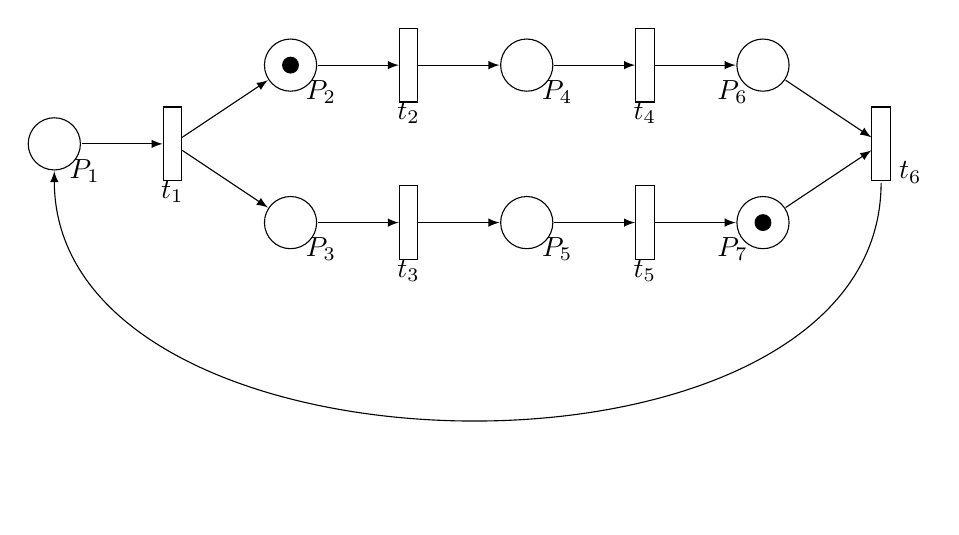
\begin{tikzpicture}
    % Liste des places
    \draw (-6,0) node[below right = 2pt] {$P_1$};
    \node[draw,circle,scale=2] (P1) at (-6, 0) {};
    \draw (-3,1) node[below right = 2pt] {$P_2$};
    \node[draw,circle,scale=2] (P2) at (-3, 1) {};
    \draw (-3,-1) node[below right = 2pt] {$P_3$};
    \node[draw,circle,scale=2] (P3) at (-3,-1) {};
    \draw (0,1) node[below right = 2pt] {$P_4$};
    \node[draw,circle,scale=2] (P4) at (0, 1) {};
    \draw (0,-1) node[below right = 2pt] {$P_5$};
    \node[draw,circle,scale=2] (P5) at (0,-1) {};
    \draw (3,1) node[below left = 2pt] {$P_6$};
    \node[draw,circle,scale=2] (P6) at (3, 1) {};
    \draw (3,-1) node[below left = 2pt] {$P_7$};
    \node[draw,circle,scale=2] (P7) at (3,-1) {};

    % Liste des transitions
    \draw (-4.5,0) node[below = 10pt] {$t_1$};
    \node[draw,rectangle,yscale=4] (t1) at (-4.5, 0) {};
    \draw (-1.5,-1) node[below = 10pt] {$t_3$};
    \node[draw,rectangle,yscale=4] (t3) at (-1.5, -1) {};
    \draw (-1.5,1) node[below = 10pt] {$t_2$};
    \node[draw,rectangle,yscale=4] (t2) at (-1.5, 1) {};
    \draw (1.5,-1) node[below = 10pt] {$t_5$};
    \node[draw,rectangle,yscale=4] (t5) at (1.5, -1) {};
    \draw (1.5,1) node[below = 10pt] {$t_4$};
    \node[draw,rectangle,yscale=4] (t4) at (1.5, 1) {};
    \draw (4.5,0) node[below right= 3pt] {$t_6$};
    \node[draw,rectangle,yscale=4] (t6) at (4.5, 0) {};

    % Liste des arcs
    \draw[->,>=latex] (P1) -- (t1);
    \draw[->,>=latex] (t1) -- (P2);
    \draw[->,>=latex] (t1) -- (P3);
    \draw[->,>=latex] (P3) -- (t3);
    \draw[->,>=latex] (P2) -- (t2);
    \draw[->,>=latex] (t2) -- (P4);
    \draw[->,>=latex] (t3) -- (P5);
    \draw[->,>=latex] (P4) -- (t4);
    \draw[->,>=latex] (P5) -- (t5);
    \draw[->,>=latex] (t4) -- (P6);
    \draw[->,>=latex] (t5) -- (P7);
    \draw[->,>=latex] (P6) -- (t6);
    \draw[->,>=latex] (P7) -- (t6);
    \draw[->,>=latex] (t6) to[out=-90,in=-90] (P1);

    % Marquage 
    \draw [fill](-3,1) circle (0.1) ;
    \draw [fill](3,-1) circle (0.1) ;
  \end{tikzpicture}
  \caption{Réseau après l'avancement et retour du pochoir gauche} \label{fig:M6}
\end{figure}

\begin{figure}[H]
  \centering
  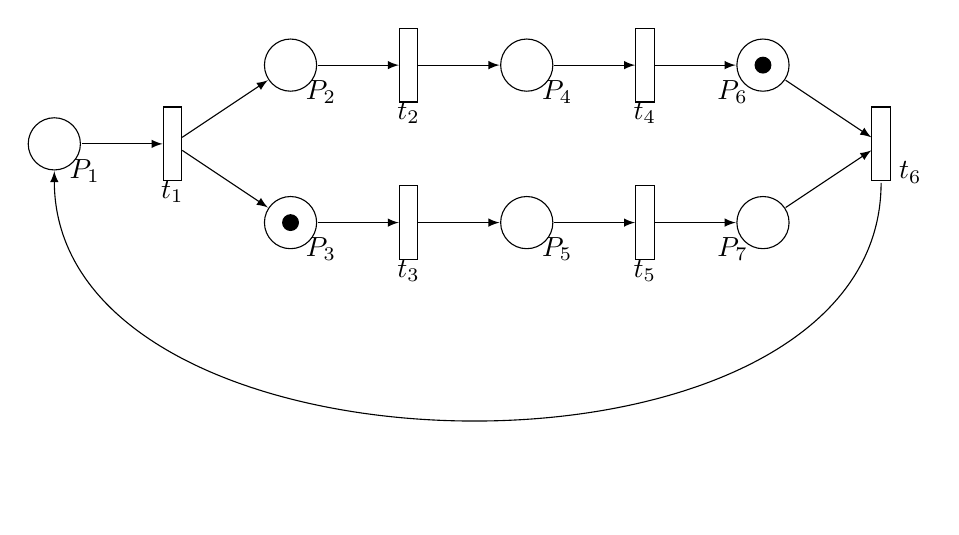
\begin{tikzpicture}
    % Liste des places
    \draw (-6,0) node[below right = 2pt] {$P_1$};
    \node[draw,circle,scale=2] (P1) at (-6, 0) {};
    \draw (-3,1) node[below right = 2pt] {$P_2$};
    \node[draw,circle,scale=2] (P2) at (-3, 1) {};
    \draw (-3,-1) node[below right = 2pt] {$P_3$};
    \node[draw,circle,scale=2] (P3) at (-3,-1) {};
    \draw (0,1) node[below right = 2pt] {$P_4$};
    \node[draw,circle,scale=2] (P4) at (0, 1) {};
    \draw (0,-1) node[below right = 2pt] {$P_5$};
    \node[draw,circle,scale=2] (P5) at (0,-1) {};
    \draw (3,1) node[below left = 2pt] {$P_6$};
    \node[draw,circle,scale=2] (P6) at (3, 1) {};
    \draw (3,-1) node[below left = 2pt] {$P_7$};
    \node[draw,circle,scale=2] (P7) at (3,-1) {};

    % Liste des transitions
    \draw (-4.5,0) node[below = 10pt] {$t_1$};
    \node[draw,rectangle,yscale=4] (t1) at (-4.5, 0) {};
    \draw (-1.5,-1) node[below = 10pt] {$t_3$};
    \node[draw,rectangle,yscale=4] (t3) at (-1.5, -1) {};
    \draw (-1.5,1) node[below = 10pt] {$t_2$};
    \node[draw,rectangle,yscale=4] (t2) at (-1.5, 1) {};
    \draw (1.5,-1) node[below = 10pt] {$t_5$};
    \node[draw,rectangle,yscale=4] (t5) at (1.5, -1) {};
    \draw (1.5,1) node[below = 10pt] {$t_4$};
    \node[draw,rectangle,yscale=4] (t4) at (1.5, 1) {};
    \draw (4.5,0) node[below right= 3pt] {$t_6$};
    \node[draw,rectangle,yscale=4] (t6) at (4.5, 0) {};

    % Liste des arcs
    \draw[->,>=latex] (P1) -- (t1);
    \draw[->,>=latex] (t1) -- (P2);
    \draw[->,>=latex] (t1) -- (P3);
    \draw[->,>=latex] (P3) -- (t3);
    \draw[->,>=latex] (P2) -- (t2);
    \draw[->,>=latex] (t2) -- (P4);
    \draw[->,>=latex] (t3) -- (P5);
    \draw[->,>=latex] (P4) -- (t4);
    \draw[->,>=latex] (P5) -- (t5);
    \draw[->,>=latex] (t4) -- (P6);
    \draw[->,>=latex] (t5) -- (P7);
    \draw[->,>=latex] (P6) -- (t6);
    \draw[->,>=latex] (P7) -- (t6);
    \draw[->,>=latex] (t6) to[out=-90,in=-90] (P1);

    % Marquage 
    \draw [fill](3,1) circle (0.1) ;
    \draw [fill](-3,-1) circle (0.1) ;
  \end{tikzpicture}
  \caption{Réseau après l'avancement et le retour du pochoir droit} \label{fig:M7}
\end{figure}

On obtient ainsi de plus en plus de cas à étudier :\\
\begin{enumerate}
  \item Si on a fait avancer et reculer le pochoir droit
    \begin{itemize}
      \item On doit alors faire avancer le pochoir gauche : fig. 9
    \end{itemize}
  \item Si on a fait avancer et reculer le pochoir gauche
    \begin{itemize}
      \item On doit alors faire avancer le pochoir droit : fig. 8
    \end{itemize}
  \item Si on a fait avancer les deux pochoirs
    \begin{itemize}
      \item On doit alors faire reculer l'un des deux pochoirs
        \begin{itemize}
          \item pochoir droit : fig. 9
          \item pochoir gauche : fig. 8
        \end{itemize}
   \end{itemize}
\end{enumerate}


\begin{figure}[H]
  \centering
  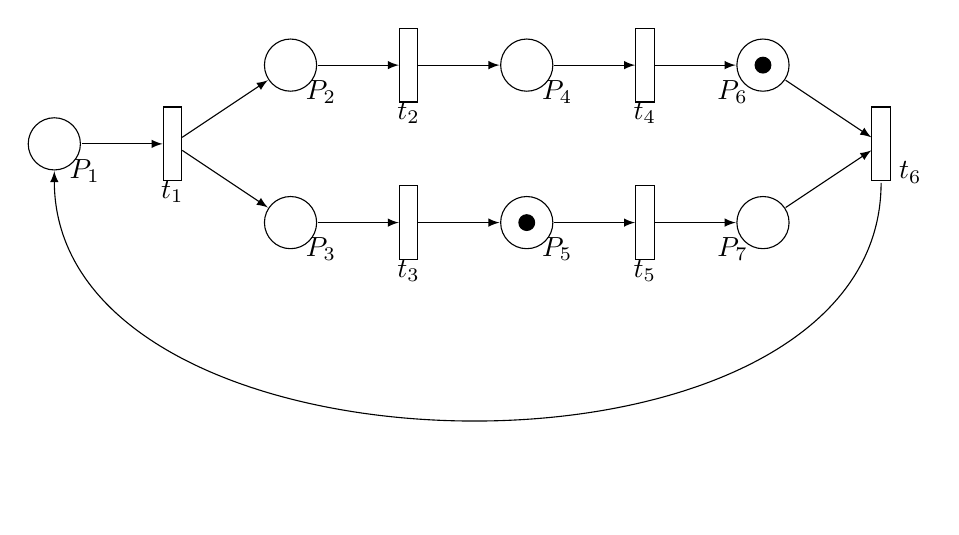
\begin{tikzpicture}
    % Liste des places
    \draw (-6,0) node[below right = 2pt] {$P_1$};
    \node[draw,circle,scale=2] (P1) at (-6, 0) {};
    \draw (-3,1) node[below right = 2pt] {$P_2$};
    \node[draw,circle,scale=2] (P2) at (-3, 1) {};
    \draw (-3,-1) node[below right = 2pt] {$P_3$};
    \node[draw,circle,scale=2] (P3) at (-3,-1) {};
    \draw (0,1) node[below right = 2pt] {$P_4$};
    \node[draw,circle,scale=2] (P4) at (0, 1) {};
    \draw (0,-1) node[below right = 2pt] {$P_5$};
    \node[draw,circle,scale=2] (P5) at (0,-1) {};
    \draw (3,1) node[below left = 2pt] {$P_6$};
    \node[draw,circle,scale=2] (P6) at (3, 1) {};
    \draw (3,-1) node[below left = 2pt] {$P_7$};
    \node[draw,circle,scale=2] (P7) at (3,-1) {};

    % Liste des transitions
    \draw (-4.5,0) node[below = 10pt] {$t_1$};
    \node[draw,rectangle,yscale=4] (t1) at (-4.5, 0) {};
    \draw (-1.5,-1) node[below = 10pt] {$t_3$};
    \node[draw,rectangle,yscale=4] (t3) at (-1.5, -1) {};
    \draw (-1.5,1) node[below = 10pt] {$t_2$};
    \node[draw,rectangle,yscale=4] (t2) at (-1.5, 1) {};
    \draw (1.5,-1) node[below = 10pt] {$t_5$};
    \node[draw,rectangle,yscale=4] (t5) at (1.5, -1) {};
    \draw (1.5,1) node[below = 10pt] {$t_4$};
    \node[draw,rectangle,yscale=4] (t4) at (1.5, 1) {};
    \draw (4.5,0) node[below right= 3pt] {$t_6$};
    \node[draw,rectangle,yscale=4] (t6) at (4.5, 0) {};

    % Liste des arcs
    \draw[->,>=latex] (P1) -- (t1);
    \draw[->,>=latex] (t1) -- (P2);
    \draw[->,>=latex] (t1) -- (P3);
    \draw[->,>=latex] (P3) -- (t3);
    \draw[->,>=latex] (P2) -- (t2);
    \draw[->,>=latex] (t2) -- (P4);
    \draw[->,>=latex] (t3) -- (P5);
    \draw[->,>=latex] (P4) -- (t4);
    \draw[->,>=latex] (P5) -- (t5);
    \draw[->,>=latex] (t4) -- (P6);
    \draw[->,>=latex] (t5) -- (P7);
    \draw[->,>=latex] (P6) -- (t6);
    \draw[->,>=latex] (P7) -- (t6);
    \draw[->,>=latex] (t6) to[out=-90,in=-90] (P1);

    % Marquage 
    \draw [fill](3,1) circle (0.1) ;
    \draw [fill](0,-1) circle (0.1) ;
  \end{tikzpicture}
  \caption{Réseau après l'avancement des 2 pochoirs et le retour du pochoir droit} \label{fig:M8}
\end{figure}

\begin{figure}[H]
  \centering
  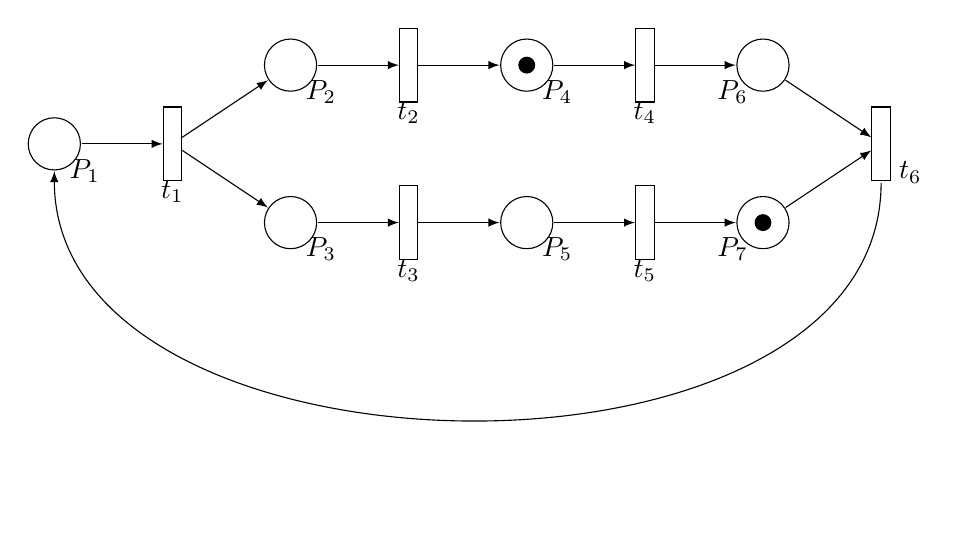
\begin{tikzpicture}
    % Liste des places
    \draw (-6,0) node[below right = 2pt] {$P_1$};
    \node[draw,circle,scale=2] (P1) at (-6, 0) {};
    \draw (-3,1) node[below right = 2pt] {$P_2$};
    \node[draw,circle,scale=2] (P2) at (-3, 1) {};
    \draw (-3,-1) node[below right = 2pt] {$P_3$};
    \node[draw,circle,scale=2] (P3) at (-3,-1) {};
    \draw (0,1) node[below right = 2pt] {$P_4$};
    \node[draw,circle,scale=2] (P4) at (0, 1) {};
    \draw (0,-1) node[below right = 2pt] {$P_5$};
    \node[draw,circle,scale=2] (P5) at (0,-1) {};
    \draw (3,1) node[below left = 2pt] {$P_6$};
    \node[draw,circle,scale=2] (P6) at (3, 1) {};
    \draw (3,-1) node[below left = 2pt] {$P_7$};
    \node[draw,circle,scale=2] (P7) at (3,-1) {};

    % Liste des transitions
    \draw (-4.5,0) node[below = 10pt] {$t_1$};
    \node[draw,rectangle,yscale=4] (t1) at (-4.5, 0) {};
    \draw (-1.5,-1) node[below = 10pt] {$t_3$};
    \node[draw,rectangle,yscale=4] (t3) at (-1.5, -1) {};
    \draw (-1.5,1) node[below = 10pt] {$t_2$};
    \node[draw,rectangle,yscale=4] (t2) at (-1.5, 1) {};
    \draw (1.5,-1) node[below = 10pt] {$t_5$};
    \node[draw,rectangle,yscale=4] (t5) at (1.5, -1) {};
    \draw (1.5,1) node[below = 10pt] {$t_4$};
    \node[draw,rectangle,yscale=4] (t4) at (1.5, 1) {};
    \draw (4.5,0) node[below right= 3pt] {$t_6$};
    \node[draw,rectangle,yscale=4] (t6) at (4.5, 0) {};

    % Liste des arcs
    \draw[->,>=latex] (P1) -- (t1);
    \draw[->,>=latex] (t1) -- (P2);
    \draw[->,>=latex] (t1) -- (P3);
    \draw[->,>=latex] (P3) -- (t3);
    \draw[->,>=latex] (P2) -- (t2);
    \draw[->,>=latex] (t2) -- (P4);
    \draw[->,>=latex] (t3) -- (P5);
    \draw[->,>=latex] (P4) -- (t4);
    \draw[->,>=latex] (P5) -- (t5);
    \draw[->,>=latex] (t4) -- (P6);
    \draw[->,>=latex] (t5) -- (P7);
    \draw[->,>=latex] (P6) -- (t6);
    \draw[->,>=latex] (P7) -- (t6);
    \draw[->,>=latex] (t6) to[out=-90,in=-90] (P1);

    % Marquage 
    \draw [fill](0,1) circle (0.1) ;
    \draw [fill](3,-1) circle (0.1) ;
  \end{tikzpicture}
  \caption{Réseau après l'avancement des 2 pochoirs et le retour du pochoir gauche} \label{fig:M9}
\end{figure}

Dans les deux cas ci-dessus, il nous reste à faire reculer le pochoir qui ne l'a pas encore fait.
Et on obtient le même réseau dans les 2 cas :

\begin{figure}[H]
  \centering
  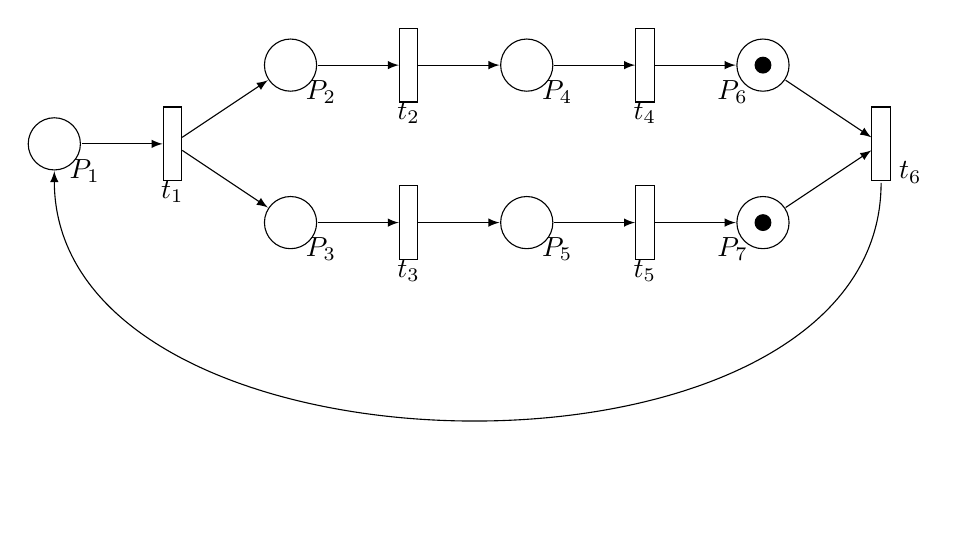
\begin{tikzpicture}
    % Liste des places
    \draw (-6,0) node[below right = 2pt] {$P_1$};
    \node[draw,circle,scale=2] (P1) at (-6, 0) {};
    \draw (-3,1) node[below right = 2pt] {$P_2$};
    \node[draw,circle,scale=2] (P2) at (-3, 1) {};
    \draw (-3,-1) node[below right = 2pt] {$P_3$};
    \node[draw,circle,scale=2] (P3) at (-3,-1) {};
    \draw (0,1) node[below right = 2pt] {$P_4$};
    \node[draw,circle,scale=2] (P4) at (0, 1) {};
    \draw (0,-1) node[below right = 2pt] {$P_5$};
    \node[draw,circle,scale=2] (P5) at (0,-1) {};
    \draw (3,1) node[below left = 2pt] {$P_6$};
    \node[draw,circle,scale=2] (P6) at (3, 1) {};
    \draw (3,-1) node[below left = 2pt] {$P_7$};
    \node[draw,circle,scale=2] (P7) at (3,-1) {};

    % Liste des transitions
    \draw (-4.5,0) node[below = 10pt] {$t_1$};
    \node[draw,rectangle,yscale=4] (t1) at (-4.5, 0) {};
    \draw (-1.5,-1) node[below = 10pt] {$t_3$};
    \node[draw,rectangle,yscale=4] (t3) at (-1.5, -1) {};
    \draw (-1.5,1) node[below = 10pt] {$t_2$};
    \node[draw,rectangle,yscale=4] (t2) at (-1.5, 1) {};
    \draw (1.5,-1) node[below = 10pt] {$t_5$};
    \node[draw,rectangle,yscale=4] (t5) at (1.5, -1) {};
    \draw (1.5,1) node[below = 10pt] {$t_4$};
    \node[draw,rectangle,yscale=4] (t4) at (1.5, 1) {};
    \draw (4.5,0) node[below right= 3pt] {$t_6$};
    \node[draw,rectangle,yscale=4] (t6) at (4.5, 0) {};

    % Liste des arcs
    \draw[->,>=latex] (P1) -- (t1);
    \draw[->,>=latex] (t1) -- (P2);
    \draw[->,>=latex] (t1) -- (P3);
    \draw[->,>=latex] (P3) -- (t3);
    \draw[->,>=latex] (P2) -- (t2);
    \draw[->,>=latex] (t2) -- (P4);
    \draw[->,>=latex] (t3) -- (P5);
    \draw[->,>=latex] (P4) -- (t4);
    \draw[->,>=latex] (P5) -- (t5);
    \draw[->,>=latex] (t4) -- (P6);
    \draw[->,>=latex] (t5) -- (P7);
    \draw[->,>=latex] (P6) -- (t6);
    \draw[->,>=latex] (P7) -- (t6);
    \draw[->,>=latex] (t6) to[out=-90,in=-90] (P1);

    % Marquage 
    \draw [fill](3,1) circle (0.1) ;
    \draw [fill](3,-1) circle (0.1) ;
  \end{tikzpicture}
  \caption{Réseau après l'avancement et le retour des 2 pochoirs} \label{fig:M10}
\end{figure}

Enfin, la piece est imprimée et le système revient à son état initiale en fig 1.

\subsection{Question 3}
Comme nous l'avons, vu en faisant évoluer le système et le reseau, chaque place ne peut recevoir qu'un jeton avec le marquage initiale $M0 = (1,0,0,0,0,0,0)$.\\
Le reseau est donc cohérent.

\subsection{Question 4}
Les signaux incompatibles, tel que $Ad \wedge \overline{Rd}$ et $\overline{Ad} \wedge Rd$, se trouve tous la même ligne du reseau, où un seul jeton navigue.
Donc si l'une de ces places possède un jeton les autres ne peuvent pas en avoir un.
Ainsi, il y a bien une exclusion mutuelle entre ces places.

\subsection{Question 5}

Nous pouvons construire le graphe de marquage suivant :

\begin{figure}[H]
  \centering
  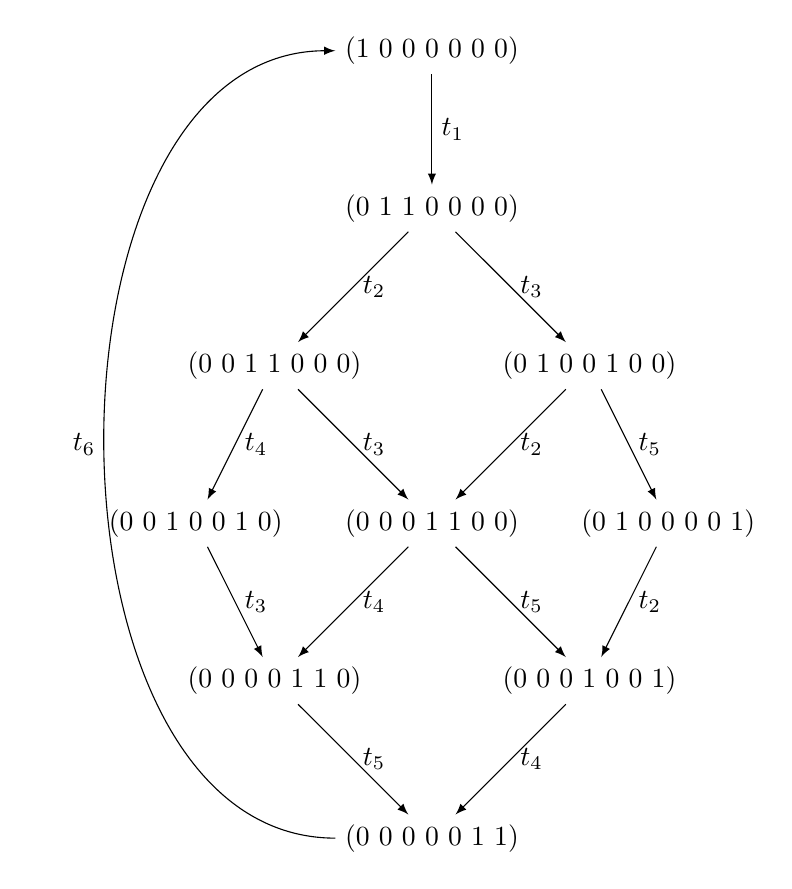
\begin{tikzpicture}
    % Liste des Marquage
    \node (M0) at (0,6) {$(1\ 0\ 0\ 0\ 0\ 0\ 0)$};
    \node (M1) at (0,4) {$(0\ 1\ 1\ 0\ 0\ 0\ 0)$};
    \node (M2) at (-2,2) {$(0\ 0\ 1\ 1\ 0\ 0\ 0)$};
    \node (M3) at (2,2) {$(0\ 1\ 0\ 0\ 1\ 0\ 0)$};
    \node (M4) at (-3,0) {$(0\ 0\ 1\ 0\ 0\ 1\ 0)$};
    \node (M5) at (0,0) {$(0\ 0\ 0\ 1\ 1\ 0\ 0)$};
    \node (M6) at (3,0) {$(0\ 1\ 0\ 0\ 0\ 0\ 1)$};
    \node (M7) at (-2,-2) {$(0\ 0\ 0\ 0\ 1\ 1\ 0)$};
    \node (M8) at (2,-2) {$(0\ 0\ 0\ 1\ 0\ 0\ 1)$};
    \node (M9) at (0,-4) {$(0\ 0\ 0\ 0\ 0\ 1\ 1)$};

     % Liste des arcs
    \draw[->,>=latex] (M0) -- (M1) node[midway, right]{$t_1$};
    \draw[->,>=latex] (M1) -- (M2) node[midway, right]{$t_2$};
    \draw[->,>=latex] (M1) -- (M3) node[midway, right]{$t_3$};
    \draw[->,>=latex] (M2) -- (M4) node[midway, right]{$t_4$};
    \draw[->,>=latex] (M2) -- (M5) node[midway, right]{$t_3$};
    \draw[->,>=latex] (M3) -- (M5) node[midway, right]{$t_2$};
    \draw[->,>=latex] (M3) -- (M6) node[midway, right]{$t_5$};
    \draw[->,>=latex] (M4) -- (M7) node[midway, right]{$t_3$};
    \draw[->,>=latex] (M5) -- (M7) node[midway, right]{$t_4$};
    \draw[->,>=latex] (M5) -- (M8) node[midway, right]{$t_5$};
    \draw[->,>=latex] (M6) -- (M8) node[midway, right]{$t_2$};
    \draw[->,>=latex] (M7) -- (M9) node[midway, right]{$t_5$};
    \draw[->,>=latex] (M8) -- (M9) node[midway, right]{$t_4$};
    \draw[->,>=latex] (M9)  to[out=180,in=180] node[midway, left]{$t_6$} (M0);

  \end{tikzpicture}
  \caption{Graphe des marquages accessibles} \label{fig:M10}
\end{figure}

\vspace{1cm}

Ceci est confirmé par le logiciel TINA :
\begin{center}
  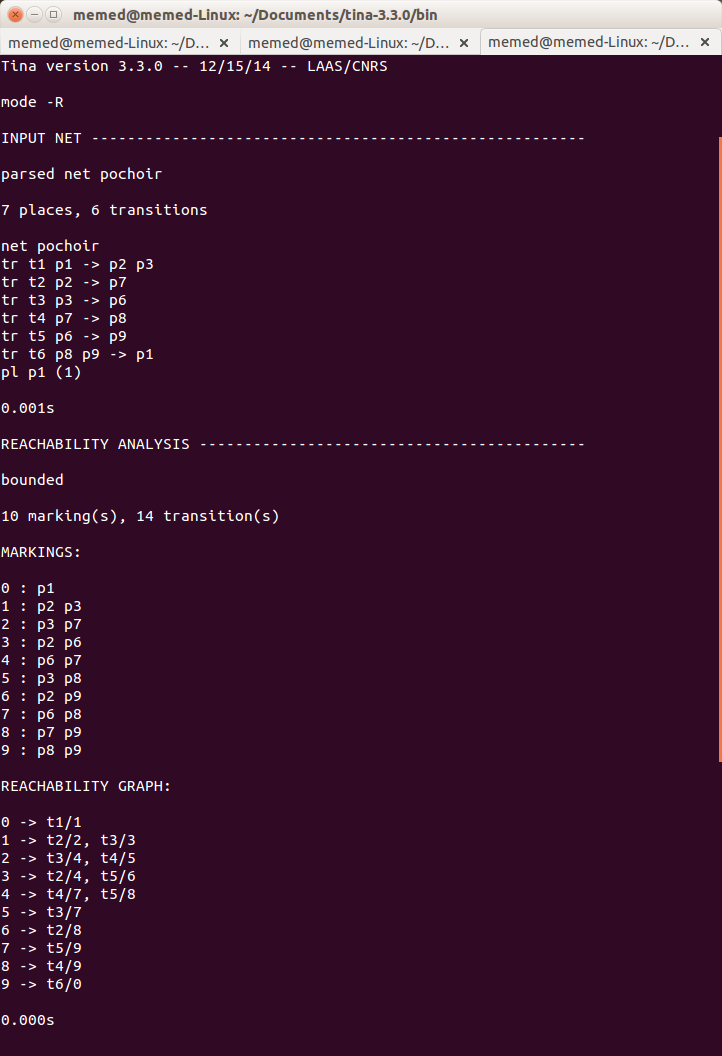
\includegraphics[width=0.25\textwidth]{images/marquage_pochoir.png}
\end{center}

\subsection{Question 6}

\vspace{1cm}

\begin{center}

{\Huge C}\qquad =\qquad $\bordermatrix{
&t_1&t_2&t_3&t_4&t_5&t_6\cr
P_1&-1&0&0&0&0&1\cr
P_2&1&-1&0&0&0&0\cr
P_3&1&0&-1&0&0&0\cr
P_4&0&1&0&-1&0&0\cr
P_5&0&0&1&0&-1&0\cr
P_6&0&0&0&1&0&-1\cr
P_7&0&0&0&0&1&-1\cr
}$

\end{center}

\subsection{Question 7}
On va utiliser l'algorithme de Farkas pour calculer les P-semi flots.

\begin{center}

$\bordermatrix{
&t_1&t_2&t_3&t_4&t_5&t_6\cr
P_1&-1&0&0&0&0&1\cr
P_2&1&-1&0&0&0&0\cr
P_3&1&0&-1&0&0&0\cr
P_4&0&1&0&-1&0&0\cr
P_5&0&0&1&0&-1&0\cr
P_6&0&0&0&1&0&-1\cr
P_7&0&0&0&0&1&-1\cr
}$

{\Huge $\downarrow$}

$\bordermatrix{
&t_1&t_2&t_3&t_4&t_5&t_6\cr
P_1+P_2&0&-1&0&0&0&1\cr
P_1+P_3&0&0&-1&0&0&1\cr
P_4&0&1&0&-1&0&0\cr
P_5&0&0&1&0&-1&0\cr
P_6&0&0&0&1&0&-1\cr
P_7&0&0&0&0&1&-1\cr
}$

{\Huge $\downarrow$}

$\bordermatrix{
&t_1&t_2&t_3&t_4&t_5&t_6\cr
P_1+P_2+P_4&0&0&0&-1&0&1\cr
P_1+P_3&0&0&-1&0&0&1\cr
P_5&0&0&1&0&-1&0\cr
P_6&0&0&0&1&0&-1\cr
P_7&0&0&0&0&1&-1\cr
}$

{\Huge $\downarrow$}

$\bordermatrix{
&t_1&t_2&t_3&t_4&t_5&t_6\cr
P_1+P_2+P_4+P_6&0&0&0&0&0&0\cr
P_1+P_3+P_5+P_7&0&0&0&0&0&0\cr
}$

\vspace{1cm}

On trouve donc 2 P-semi flots :\\
$f_1 = (1\ 1\ 0\ 1\ 0\ 1\ 0)$\\
$f_2 = (1\ 0\ 1\ 0\ 1\ 0\ 1)$

\end{center}

Ceci est confirmé par le logiciel TINA :
\begin{center}
  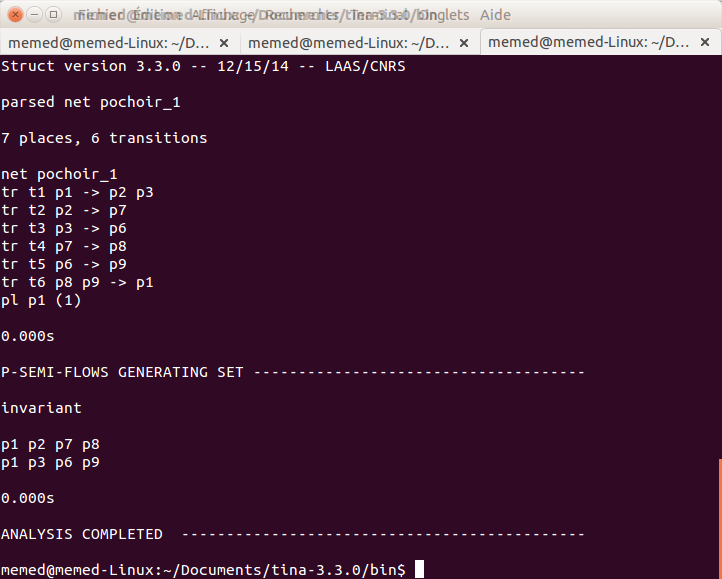
\includegraphics[width=0.25\textwidth]{images/pflot_pochoir.png}
\end{center}

\subsection{Question 8}

Soit $\{M\}$ l'ensemble des marquages accessibles du reseau.\\
Soit $\{t\}$ l'ensemble des transitions du reseau.\\
Le graphe des marquages étant sans feuille, c'est à dire que $\forall M_i \in \{M\}\ \exists t_k \in\{t\} : M_i[t_k>M_j\ avec\ M_j\in \{M\}$ \\
Le réseau est donc sans blocage.

\subsection{Question 9}

\begin{itemize}
  \item Chaque place $P_i$ possède une et une seule transition d'entrée et une et une seule transition de sortie, donc le réseau est un graphe d'événement.
  \item $s_1 = P_1 \rightarrow P_2 \rightarrow P_4 \rightarrow P_6 \rightarrow P_1$ est un circuit élémentaire
  \item $s_2 = P_1 \rightarrow P_3 \rightarrow P_5 \rightarrow P_7 \rightarrow P_1$ est un circuit élémentaire
\end{itemize}

\newpage
